% !TEX encoding = UTF-8
% !TEX TS-program = pdflatex
% !TEX root = ../tesi.tex

%**************************************************************
\chapter{Progettazione}
\label{cap:progettazione}
\label{sec:tecnologie-strumenti}

In questo capitolo vengono illustrate le strategie di progettazione adottate per la realizzazione del prodotto in questione. La progettazione viene descritta ad alto livello senza descrivere in dettaglio tutti i diagrammi delle classi. 

\section{Progettazione Frontend}
\label{sec:progettazione}
Come prima cosa sono stati realizzati utilizzando Figma i prototipi delle pagine da creare. In questo modo è stato possibile capire sin da subito la struttura delle pagina, rendendo cosi molto semplice la progettazione architetturale di tale pagine.
\subsection{Pagina cotenente l'editor}
Questa pagina contiene l'editor drag and drop. Per creare la struttura di questa pagina sono stati studiati diversi editor online che forniscono le stesse funzionalità(in diversi contesti). Dopo una attenta analisi delle strutture dei diversi editor online è stato concepita la seguente struttura:
\begin{figure}[!h] 
	\centering 
	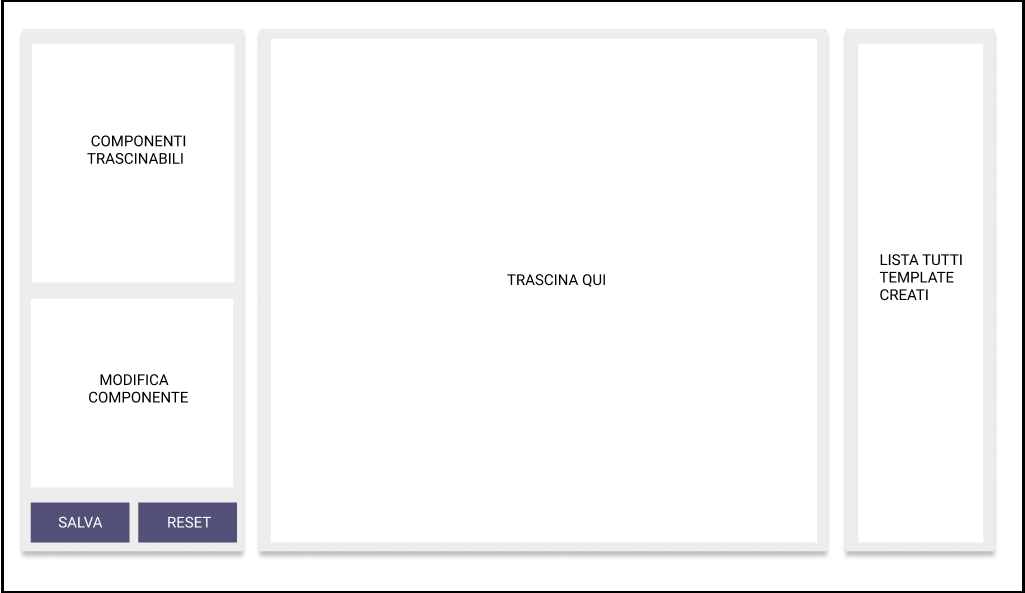
\includegraphics[width=0.9\columnwidth]{mock/mockeditor} 
	\caption{Mock pagina contenente l'editor}
\end{figure}  
\\
\begin{itemize}
	\item Il primo contenitore in alto a sinistra dovrà contenere tutti i componenti trascinabili. Ogni elemento rappresenta uno specifico tipo di oggetto HTML e CSS, come ad esempio il testo, banner, titolo, immagine ecc;
	\item Il secondo contenitore a sinistra contiene tutte le proprietà modificabili per ogni elemento;
	\item Il contenitore in centro rappresenta la zona dove tutti gli elementi vengono trascinati. In questo contenitore viene visualizzato a schermo il contenuto HTML e CSS contenuto in ogni elemento. Inoltre dovrà essere possibile modificare tale contenuto ed eliminare un elemento se necessario;
	\item Il contenitore a destra dovrà contenere tutti i template realizzati dagli utenti. Quindi esso contiene semplicemente una lista di tutti i template.  
\end{itemize}

\subsection{Pagina contenente il widget} Questa pagina contiene un semplice lista che dovrà contenere tutti i template da visualizzare nella pagina dei tickets, in modo che essa posono essere scelti dagli utenti da Zendesk.
\\ 
\subsection{Pagina login}
Semplice pagina contenete il form per il login. Una volta inseriti i valori validi l'utente sarà utenticato come amministratore, caricandoli cosi la pagina degli amministratore. 
\begin{figure}[!h] 
	\centering 
	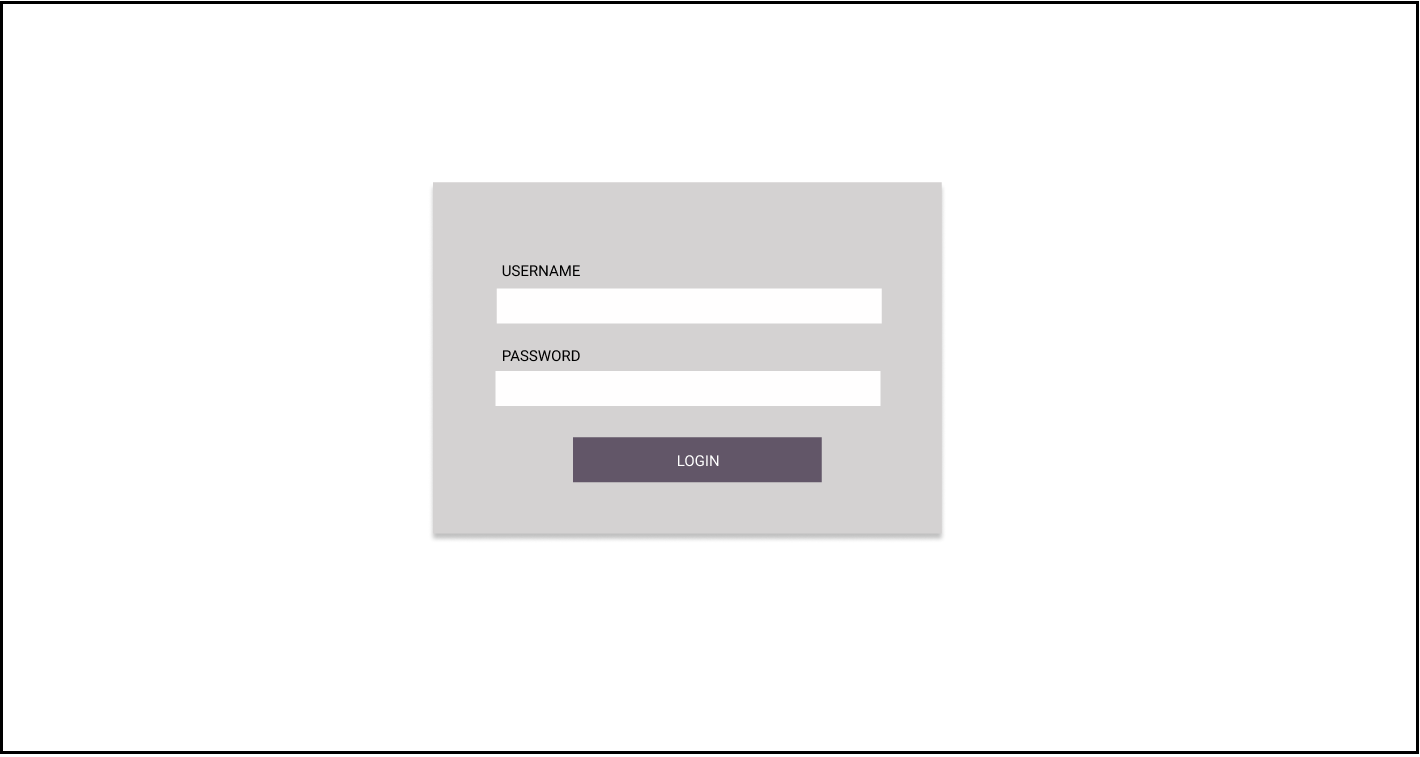
\includegraphics[width=1\columnwidth]{mock/mocklogin} 
	\caption{Mock pagina di login}
\end{figure}  \newpage
\subsection{Pagina degli amministratori}
Questa pagina dovrà essere realizzata per gli amministratore di Nextep, per permettere a loro di gestire tutti i clienti utilizzatore del applicazione. 
\begin{figure}[!h] 
	\centering 
	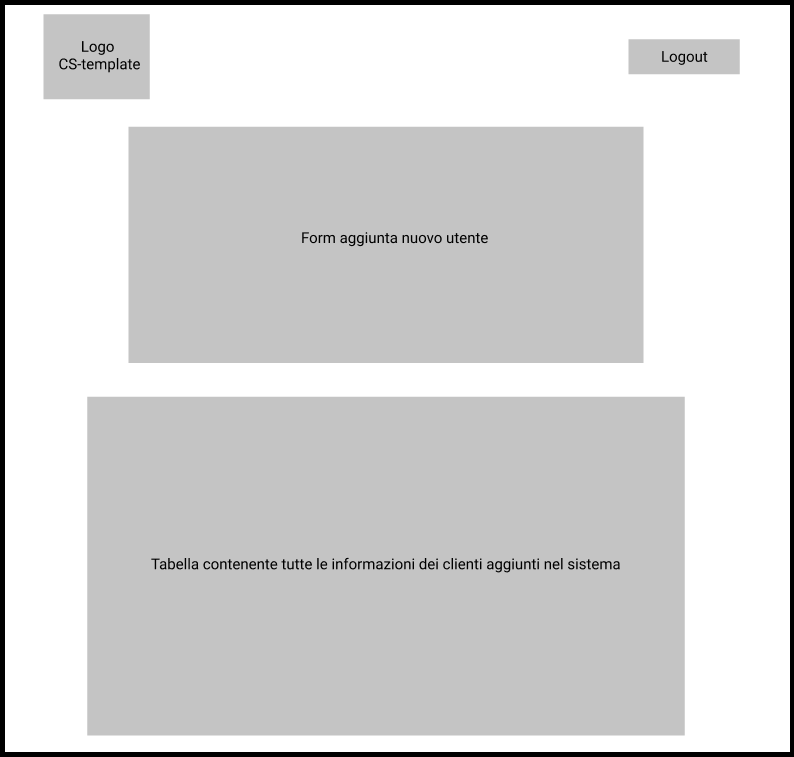
\includegraphics[width=0.8\columnwidth]{mock/mockadmin} 
	\caption{Mock pagina degli amministratori}
\end{figure} 
\newpage 
\begin{itemize}
	\item Contiene un semplice form per aggiungere un nuovo cliente;
	\item Contiene una semplice tabella, dove ogni elemento della tabella contiene le informazione di un singolo cliente.
\end{itemize}
\subsection{Struttura applicazione}
Essendo un'unica applicazione che contiene sia le pagine degli amministratore di Nextep che le pagine dell'applicazione, si è pensato quindi una struttura illustrata nel seguente diagramma.
\begin{figure}[!h] 
	\centering 
	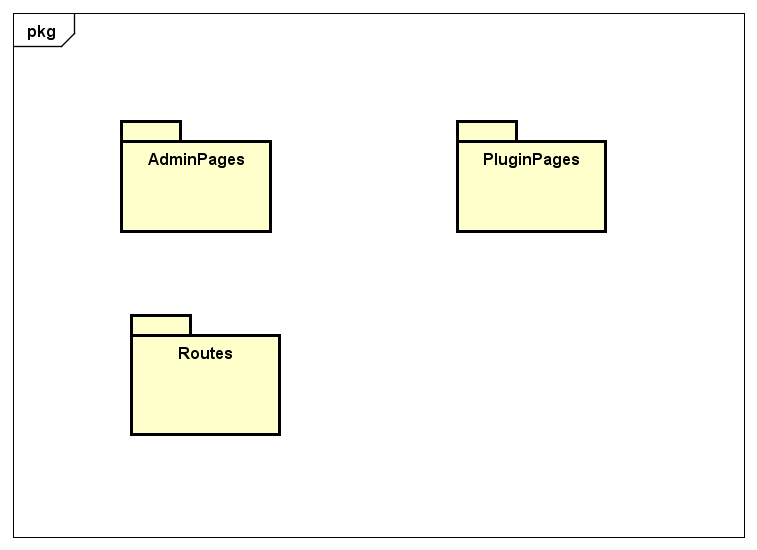
\includegraphics[width=0.8\columnwidth]{prog/pack} 
	\caption{Struttura applicazione}
\end{figure}
\begin{itemize}
	\item \textbf{AdminPages:} contiente tutti i componenti e i servizi che vanno a formare le pagine(login e di amministratori) per gli utenti di Nextep;
	\item \textbf{PluginPages:} contiene tutti i componenti e i servizi per la pagine contenente l'editor e la pagina contenente il widget;
	\item \textbf{Routes:} contiene tutto il codice per gestione della navgazione dell'applicazione.
\end{itemize}
\begin{figure}[!h] 
	\centering 
	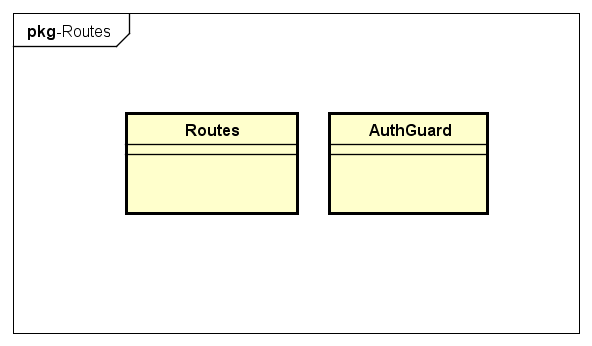
\includegraphics[width=0.7\columnwidth]{prog/routes} 
	\caption{Struttura applicazione}
\end{figure}
\begin{itemize}
	\item L'oggetto \textbf{Routes} contiene un array di tutte le navigazioni dell'applicazione,
	\item L'oggetto \textbf{AuthGuard} serve per bloccare la navigazione alla pagina degli amministratori finchè l'utente non effettua il login. 
	\\
\end{itemize}
\subsection{PluginPages}
Contiene tutti i componenti e servizi per realizzare le pagine contenente l'editor e il widget.
\begin{figure}[!h] 
	\centering 
	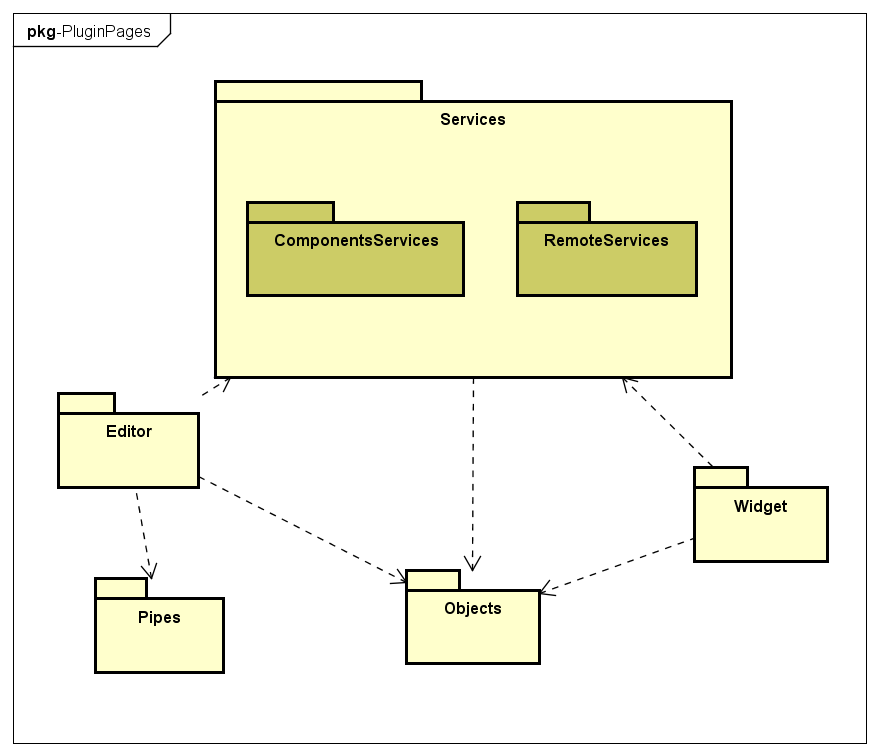
\includegraphics[width=0.8\columnwidth]{prog/pluginpages} 
	\caption{Struttura applicazione}
\end{figure}
\begin{itemize}
	\item \textbf{ComponentsServices:} contiente tutti i servizi che permettono di scambiare i dati tri componenti locali;
	\item \textbf{RemoteServices:} contiene tutti i servizi utilizzati per communicare con il lato backend dell'applicazione. Quindi principalmente per leggere, aggiungere o rimuovere i tempalte dal database su AWS;
	\item \textbf{Objects:} contiene tutti i tipi creati per rappresentare diversi tipi di dati;
	\item \textbf{Editor:} contiene tutti i componenti Angular che formano la pagine contenente l'editor;
	\item \textbf{Widget:} contiene tutti i componenti Angular che formano la pagina contenente il widget;
	\item \textbf{Pipes:} contiene le pipes di  Angular.
\end{itemize}
\newpage
\subsection{AdminPages}
Essendo un'unica applicazione che contiene sia le pagine degli amministratore di Nextep che le pagine dell'applicazione, si è pensato quindi una struttura illustrata nel seguente diagramma.
\begin{figure}[!h] 
	\centering 
	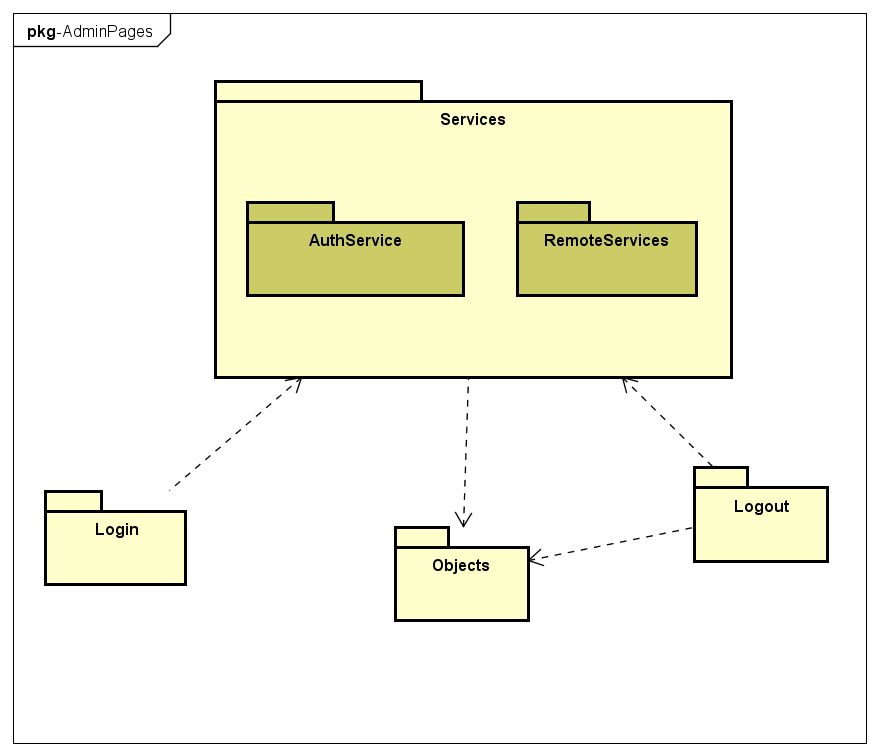
\includegraphics[width=0.8\columnwidth]{prog/adminpages} 
	\caption{Struttura applicazione}
\end{figure}
\begin{itemize}
	\item \textbf{AdminPages:} contiente tutti i componenti e i servizi che vanno a formare le pagine(login e di amministratori) per gli utenti di Nextep;
	\item \textbf{PluginPages:} contiene tutti i componenti e i servizi per la pagine contenente l'editor e la pagina contenente il widget;
	\item \textbf{Routes:} contiene tutto il codice per gestione della navgazione dell'applicazione.
\end{itemize}
\subsection{Atomic design}
Per realizzare le diverse pagine dell'applicazione è stato utilizzato il concetto di Atomic Design.
Creata da Brad Frost nel 2013, l'Atomic design è una metodologia composta da 5 differenti fasi, utile per creare un sistema di interfacce in maniera gerarchica. In questa metologia si parte dai componenti piu basilari possibili, fino ad arrivare alle pagine finali. Quindi è un approccio bottom-up.
\begin{figure}[!h] 
	\centering 
	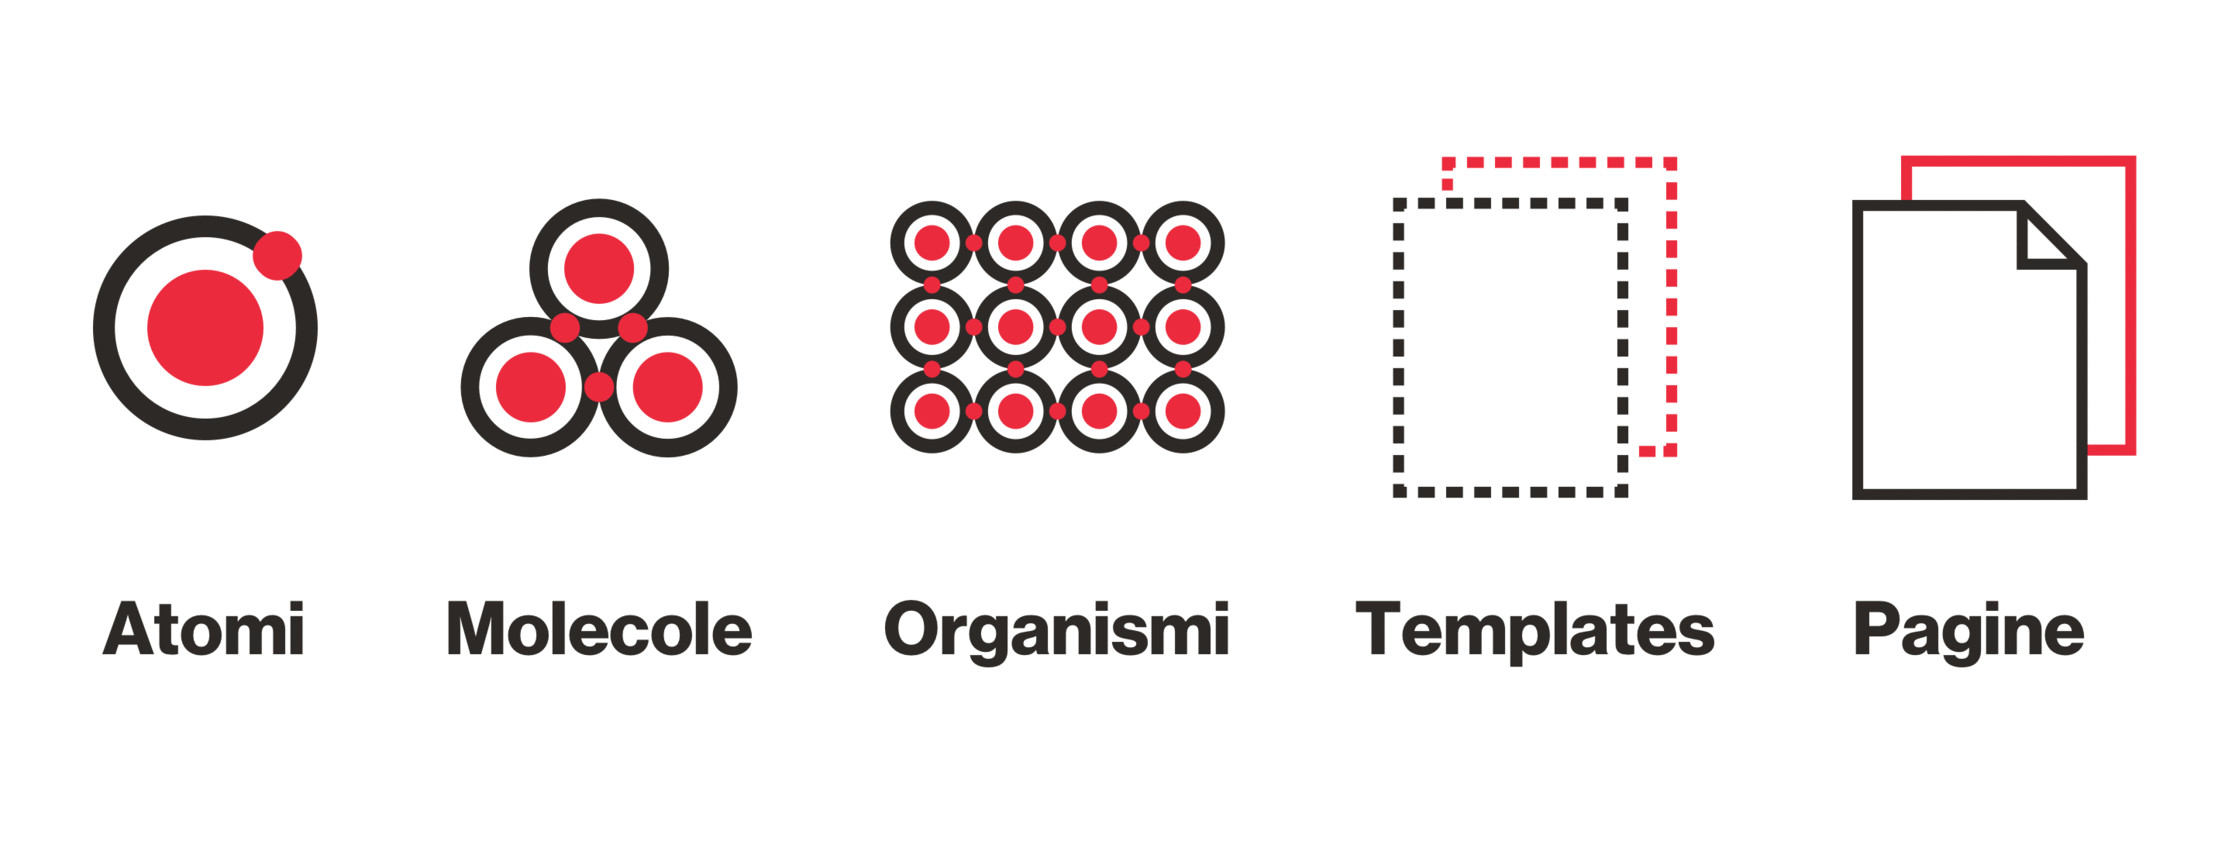
\includegraphics[width=0.8\columnwidth]{atomic} 
	\caption{Elementi atomic design}
\end{figure}
\\

\textbf{Atomi:} in fisica un atomo è la più piccola particella di un elemento che non subisce alterazioni nelle trasformazioni chimiche; nell’Atomic Design gli atomi sono i blocchi fondamentali che comprendono tutta l’interfaccia.
Questi atomi comprendono elementi HTML come tipografia, palette colori, input, bottoni e altri elementi che non possono essere suddivisi ulteriormente senza cessare di essere funzionali.
\\

\textbf{Molecole:} sono semplici gruppi di elementi d'interfaccia che funzionano uniti. Quando combiniamo due oppure più atomi, creiamo quindi una molecola.
\\

Nel contesto della applicazione gli atomi e le molecole sono rappresentate dai elementi della libreria Angular Material, che successivamente sono utilizzate per realizzare l'interfaccia di intera applicazione.

\begin{figure}[!h] 
	\centering 
	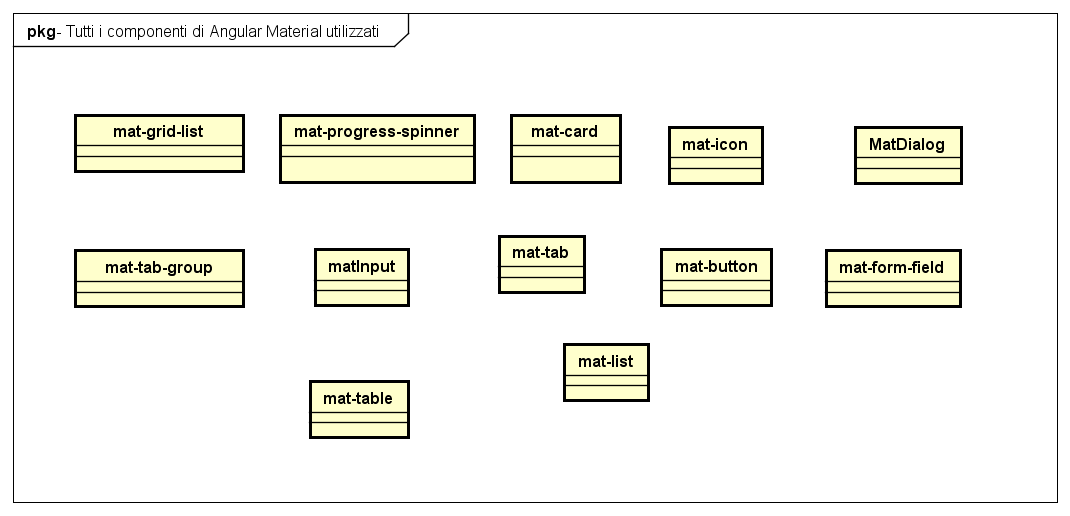
\includegraphics[width=1\columnwidth]{prog/angular} 
	\caption{Componenti Angular Material che formano gli atomi e le molecole dell'applicazione}
\end{figure} 

\textbf{Gli organismi:} sono dei componenti più o meno complessi, composti da gruppi di molecole e/o atomi e/o altri organismi. Questi organismi creano diverse sezioni all'interno della nostra interfaccia. Un esempio può essere un menu di navigazione, che è formato in media da diversi pulsanti/link. 
\\

\textbf{I templates:} sono creati dall'insieme dai nostri atomi, molecole e organismi. Creando così la prima idea di scheletro della pagina.
\\

\textbf{Le pagine:} sono dei templates riempiti di contenuto reale, come immagini, testi, elementi grafici, advertising, ecc. Una pagina quindi è formata da molti template. 
\newpage
\section{Progettazione Backend}
\subsection{Archittetura a microservizi serverless}
Il backend dell'applicazione è realizzato sutilizzando i servizi web di Amazon. I servizi scelti sono stati descritti nel capitolo 2. In questa sezione viene descritto come questi servizi communicano tra di loro. Il seguente immagine mostra la panoramica dell'archittettura della applicazione Zendesk realizzata(per la pagina degli amministratori la situazione è leggermente diversa). L'immagine di seguito descrive come un template viene caricato nel database nosql presente su Amazon. 
\begin{figure}[!h] 
	\centering 
	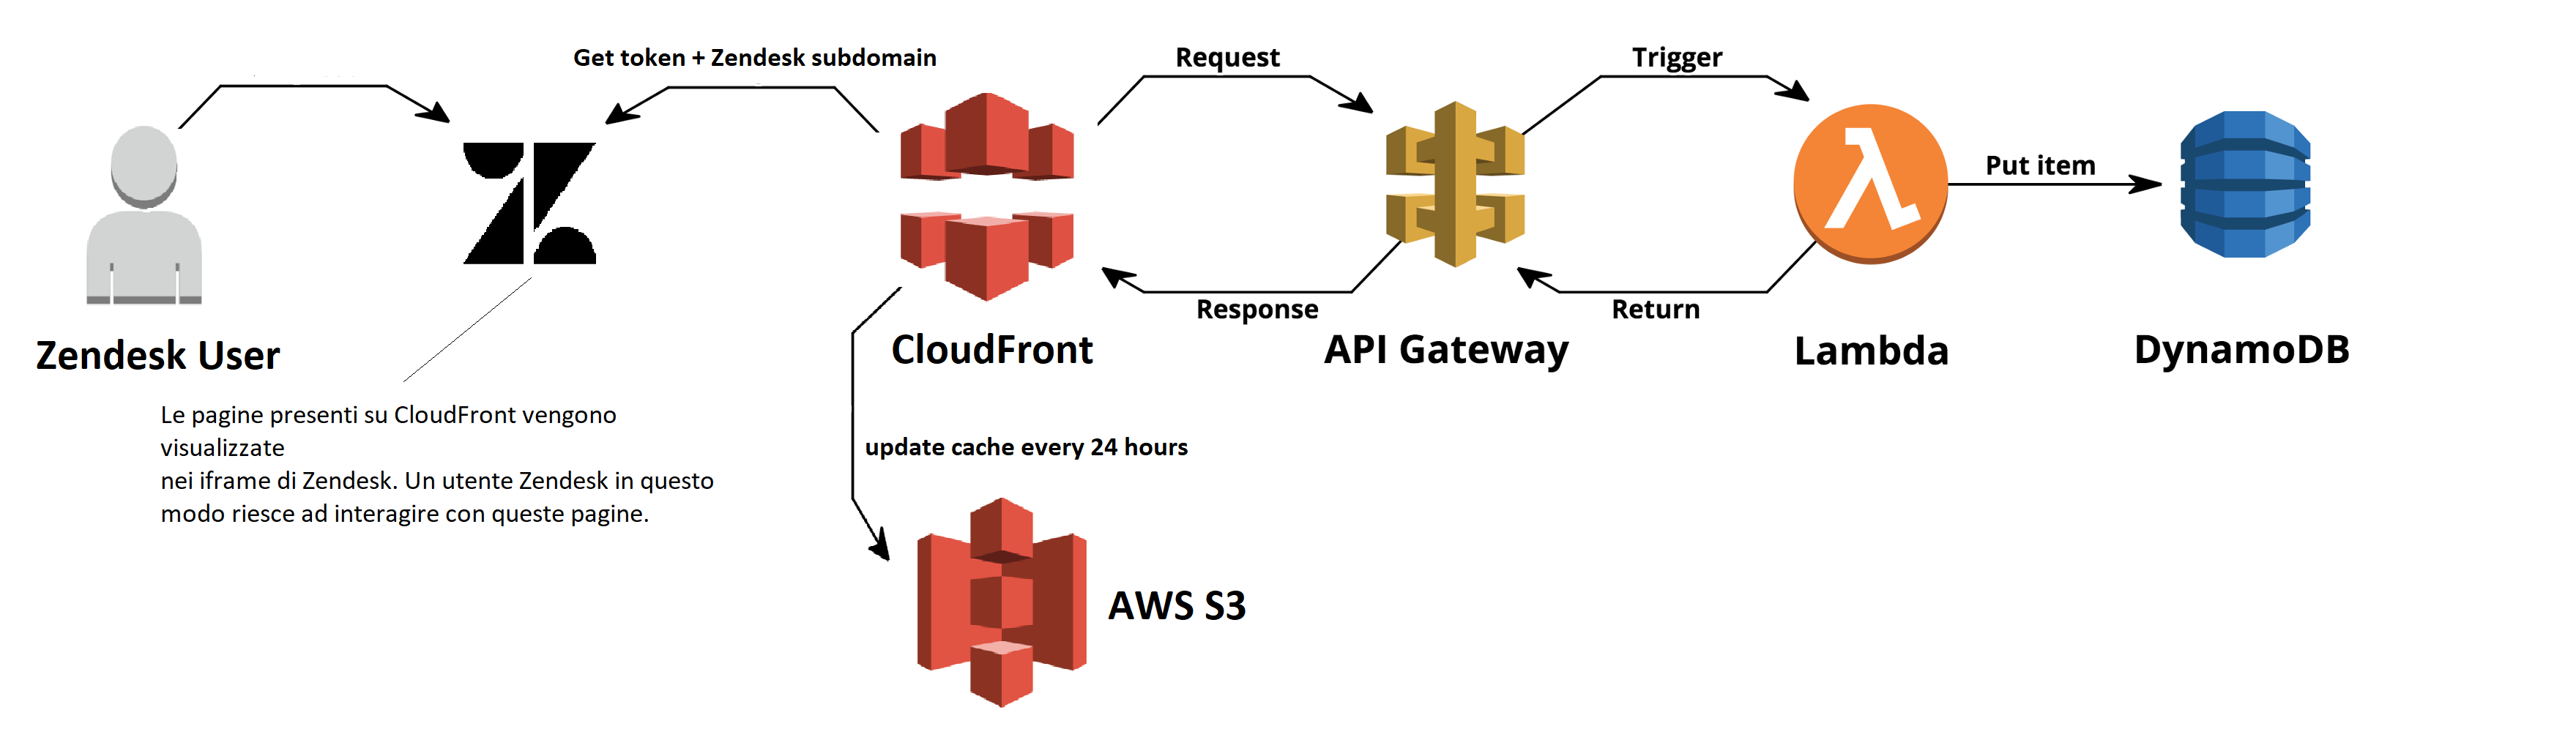
\includegraphics[width=1.2\columnwidth]{prog/zen-architecture} 
	\caption{Componenti Angular Material che formano gli atomi e le molecole dell'applicazione}
\end{figure} 
\\
\begin{itemize}
	\item Zendesk User interagisce con la applicazione tramitte l'interfaccia di Zendesk;
	\item Le pagine dell'applicazione Angular sono caricate da CloudFront sui iframe presenti su Zendesk;
	\item Le pagine appena caricate nei ifrmae leggono il token e il nome del sottodominio dalla piattforma in qui si trovano utilizzando lo oggetto ZAFClient(descritto in capitolo 2);
	\item Utente crea un nuovo template e lo salva;
	\item L'editor manda la richiesta al API Gateway inviando nel header il token e il nome del dominio;
	\item API Gateway come prima cosa verifica il token e il nome del sottodominio se sono validi. Se sono validi genera un eventi che inesa una funzione lambda altrimenti(token e nomedominio non validi) ritorna un messaggio d'erroe;
	\item La funzione lambda riceve dati dal evento generato da API Gateway. Utilizzando AWS-SDK interagisce con il database nosql e salva il nuovo item(template).
	\item Funazione lambda ritorna un messaggio di successo;
\end{itemize}
\subsection{Archittetura pagina degli amministratori}
Il backend cambia leggermente per quanto riguarda la pagina degli amministratori di Nextep. Per accedere a questa pagina bisogna effetuare il login. Il login è stato implementato utilizzanod il servizio Cognito, che permette di gestire un pool di utenti in maniera molto facile. Il seguente immagine descrive il funzionamento di questa pagina. 
\begin{figure}[!h] 
	\centering 
	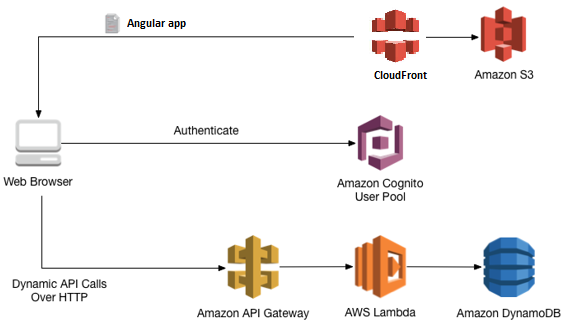
\includegraphics[width=1\columnwidth]{prog/admin-arch} 
	\caption{Archittetura }
\end{figure} 
\begin{itemize}
	\item La pagina di login viene caricato nel browser;
	\item L'utente inserisce le sue credenziali corrette per effetuare il login;
	\item AWS Cognito verifica le credenziali, se sono valide ritorna il token di accesso altrimenti un errore;
	\item Le credenziali sono valide, l'uente accede nella pagina degli amministratori;
	\item L'utente ora può communicare con il API Gateway inviando il token ritornato da AWS Cognito. Questo token permette all'utente di inserire oppure eliminare uenti dal database nosql presente su AWS;
	\item Inserimento oppure l'eliminazione di un cliente esegue stesso flusso visto sopra per il template. Tranne per il AWS Cognito la pagina degli ammministraoti ha la stessa archittetura.
\end{itemize}
